% =============================================================================
% LabFit Beamer Handout - Gaussian Peak Fitting Walkthrough
% =============================================================================
\documentclass[handout, 10pt]{beamer}

\mode<presentation>{\usetheme{default}}

\usepackage[utf8]{inputenc}
\usepackage[T1]{fontenc}
\usepackage{amsmath, amssymb}
\usepackage{booktabs}
\usepackage{graphicx}
\usepackage{listings}
\usepackage{tcolorbox}
\usepackage{xcolor}
\usepackage{hyperref}

% -----------------------------------------------------------------------------
% listings style for Python
% -----------------------------------------------------------------------------
\definecolor{codebg}{HTML}{F5F5F5}
\lstdefinestyle{pystyle}{
    language=Python,
    basicstyle=\scriptsize\ttfamily,
    backgroundcolor=\color{codebg},
    frame=single,
    rulecolor=\color{codebg!80!black},
    breaklines=true,
    columns=flexible,
    keepspaces=true,
    tabsize=4,
    showstringspaces=false,
    upquote=true,
    xleftmargin=2pt,
    xrightmargin=2pt,
}
\lstdefinestyle{pysmall}{
    style=pystyle,
    basicstyle=\tiny\ttfamily,
}

% -----------------------------------------------------------------------------
% Colour palette (Okabe-Ito)
% -----------------------------------------------------------------------------
\definecolor{labblue}{HTML}{0072B2}
\definecolor{laborange}{HTML}{D55E00}
\definecolor{labgreen}{HTML}{009E73}

\setbeamercolor{title}{fg=labblue}
\setbeamercolor{frametitle}{fg=labblue}
\setbeamercolor{structure}{fg=labblue}
\setbeamercolor{alerted text}{fg=laborange}

\setbeamertemplate{footline}[frame number]
\setbeamertemplate{navigation symbols}{}
\setbeamertemplate{itemize items}[circle]

% -----------------------------------------------------------------------------
% Title
% -----------------------------------------------------------------------------
\title{Gaussian Peak Fitting with \texttt{labfit}}
\subtitle{A Practical Walkthrough Using Mercury Emission Spectra}
\author{}
\date{}

\begin{document}

% SLIDE 1 --- Title
% =============================================================================
\begin{frame}
\maketitle

\vspace*{-12pt}
\centering
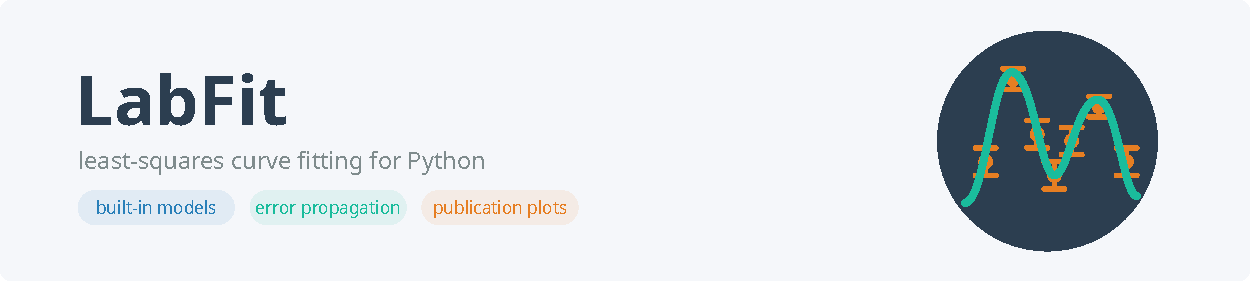
\includegraphics[width=0.85\textwidth]{data/banner.pdf}

\vspace{12pt}
\small
M.~J.~Doyle \hfill 08/06/2026

\vspace{8pt}
Covers: loading spectral data, Gaussian models, initial guesses, $\chi^2$,
multi-peak fitting, and interpreting results. \\
Library: \url{https://github.com/matthewjdoyle/labfit}
\end{frame}

% =============================================================================
% SLIDE 2 --- Spectrum basics + Gaussian model
% =============================================================================
\begin{frame}{Spectrum basics \& the Gaussian model}

\textbf{Emission spectrum:} intensity vs.\ wavelength. Each peak is an
electronic transition in the atom. Line shapes are broadened by thermal
motion (Doppler broadening).

\vspace{6pt}
\begin{columns}[t]
\begin{column}{0.46\textwidth}
\textbf{Gaussian:}
\[
I(\lambda) = A \exp\!\left[-\frac{1}{2}\left(\frac{\lambda - \lambda_0}{\sigma}\right)^{\!2}\right]
\]

\vspace{2pt}
\resizebox{\columnwidth}{!}{%
\begin{tabular}{lrl}
\toprule
Param & Meaning & Units \\
\midrule
$A$       & Peak amplitude & counts \\
$\lambda_0$ & Centre wavelength & nm \\
$\sigma$    & Width ($\sigma$) & nm \\
\bottomrule
\end{tabular}%
}
\end{column}
\begin{column}{0.42\textwidth}
\alert{Why fit?}\\
Noise shifts the apparent maximum; the true centre lies between pixels.
Fitting uses \emph{all} data points and gives rigorous uncertainties.

\vspace{6pt}
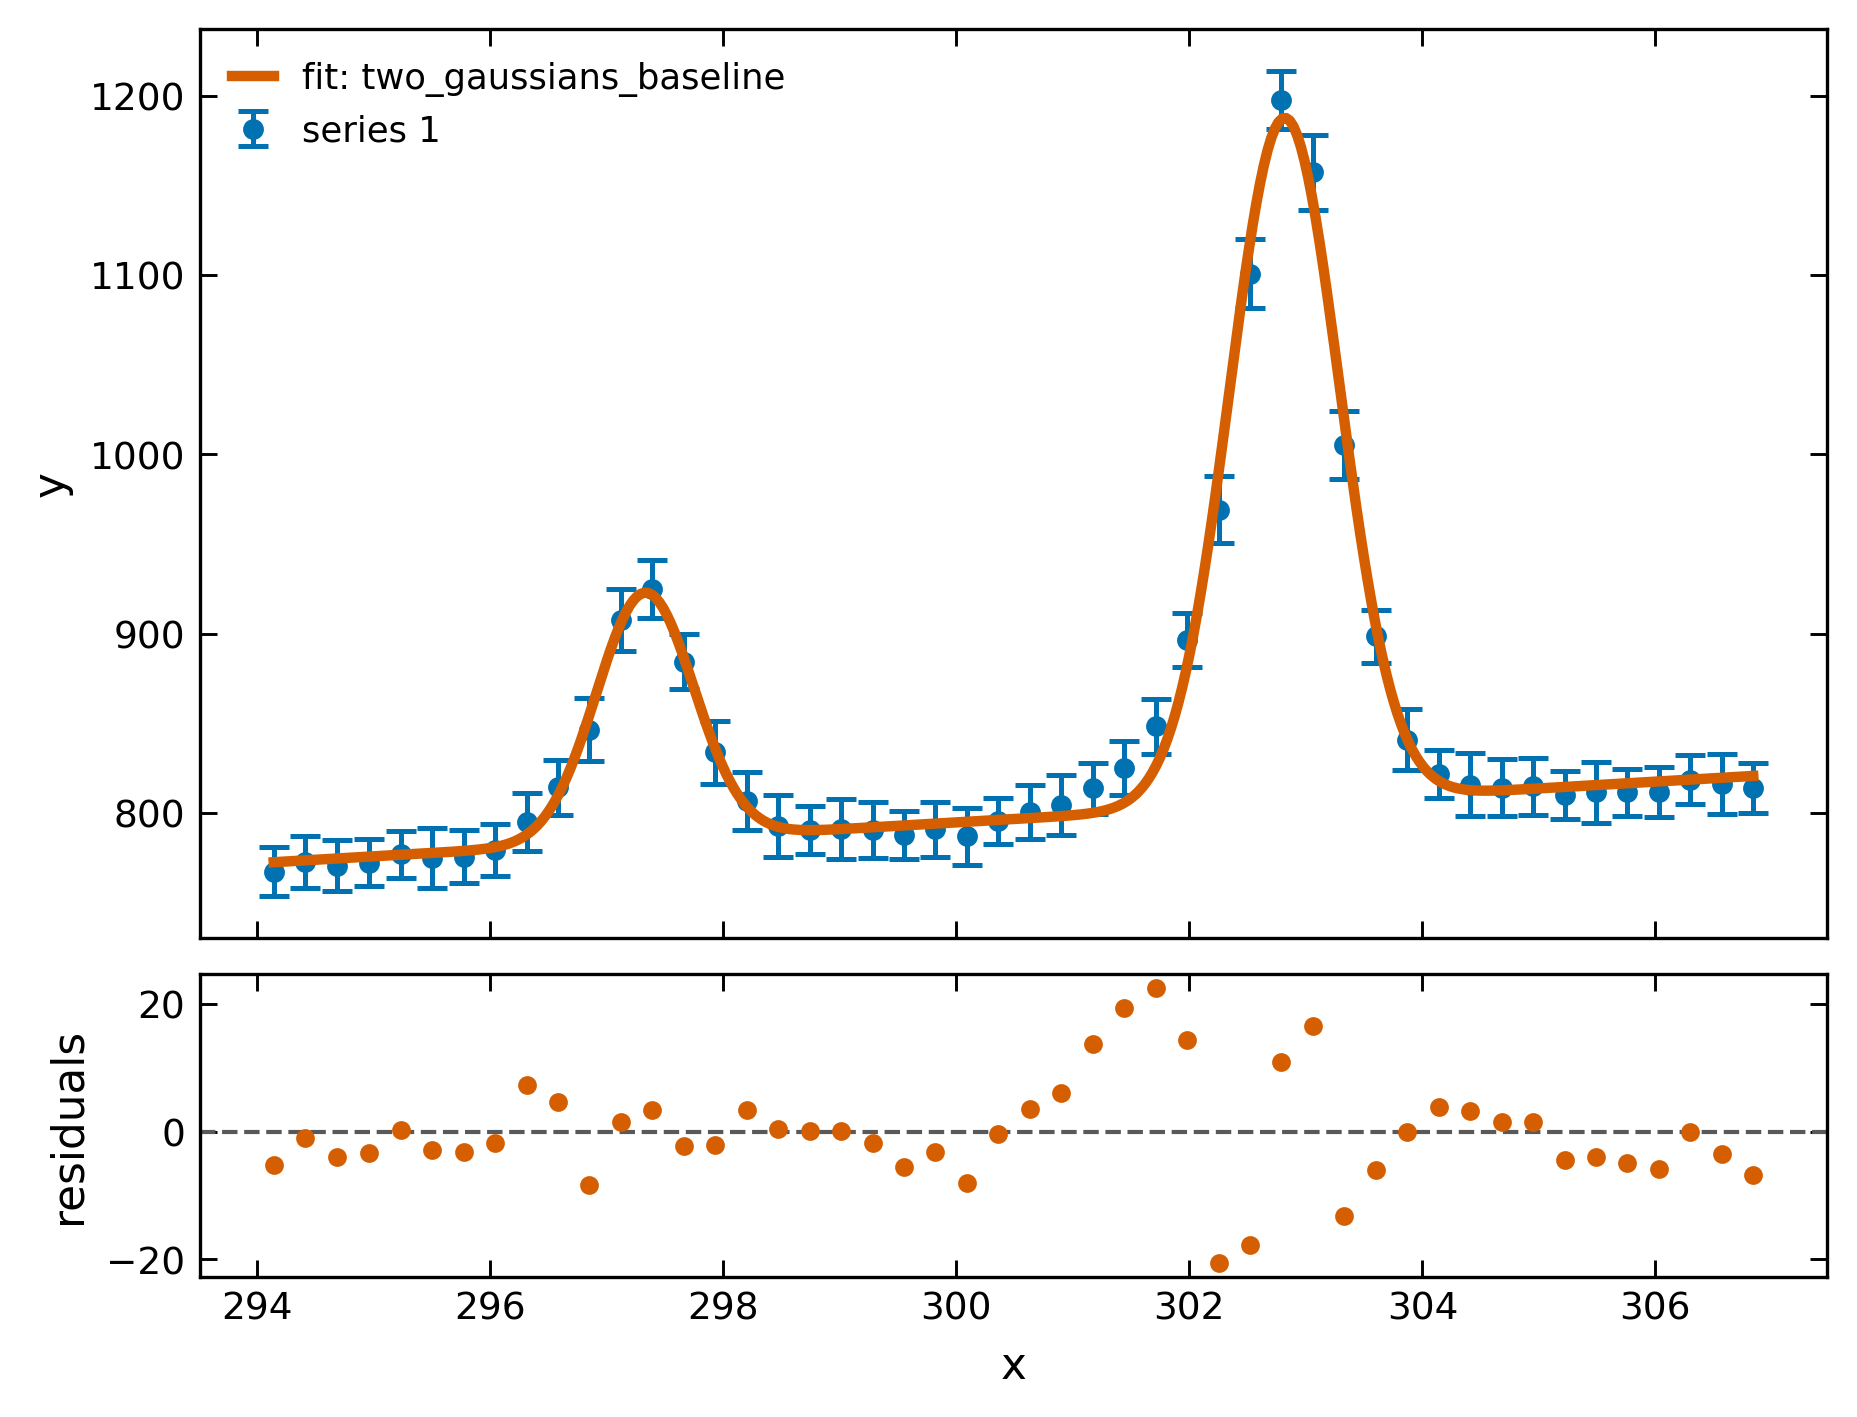
\includegraphics[width=\columnwidth]{data/mercury_300nm_bimodal_fit.png}
\end{column}
\end{columns}
\end{frame}

% =============================================================================
% SLIDE 3 --- Gaussian with baseline
% =============================================================================
\begin{frame}{Gaussian with baseline}

Real spectra sit on a background (stray light, dark current). Add a linear term:

\[
I(\lambda) = A \exp\!\left[-\frac{1}{2}\left(\frac{\lambda - \lambda_0}{\sigma}\right)^{\!2}\right]
+ m\lambda + b
\]

\medskip
\begin{center}
\begin{tabular}{lll}
\toprule
Model in \texttt{labfit} & Parameters \\
\midrule
\texttt{gaussian\_baseline} & \texttt{amplitude, mean, sigma, m, b} \\
\bottomrule
\end{tabular}
\end{center}

\medskip
\textbf{Workflow:} Load CSV $\rightarrow$ Select peak region $\rightarrow$ Fit $\rightarrow$ Plot \& interpret.
\end{frame}

% =============================================================================
% SLIDE 4 --- Load \& select
% =============================================================================
\begin{frame}[fragile]{Step 1--2: Load data \& select a peak region}

\begin{columns}[c]
\begin{column}{0.48\textwidth}
\begin{lstlisting}[style=pysmall]
from labfit.io import load_csv
from labfit import fit, plot_fit

data = load_csv("mercury_int10s.csv",
                x_col="wavelength_nm",
                y_col="intensity",
                y_err_col="y_error")
\end{lstlisting}

\tiny Output: 3648~pts, 192--1130~nm, max~16383~counts.

\begin{lstlisting}[style=pysmall]
import numpy as np

mask = (data.x > 294) & (data.x < 307)
x_pk = data.x[mask]
y_pk = data.y[mask]
e_pk = data.y_err[mask]
\end{lstlisting}

\tiny Only $\sim$48 points covering two small peaks.

\vspace{6pt}
\tiny
CSV could also be loaded with \texttt{numpy.loadtxt} or \texttt{pandas.read\_csv}; \texttt{labfit.io.load\_csv} is a convenience wrapper that preserves column names and detects error columns.
\end{column}
\begin{column}{0.46\textwidth}
\vfill
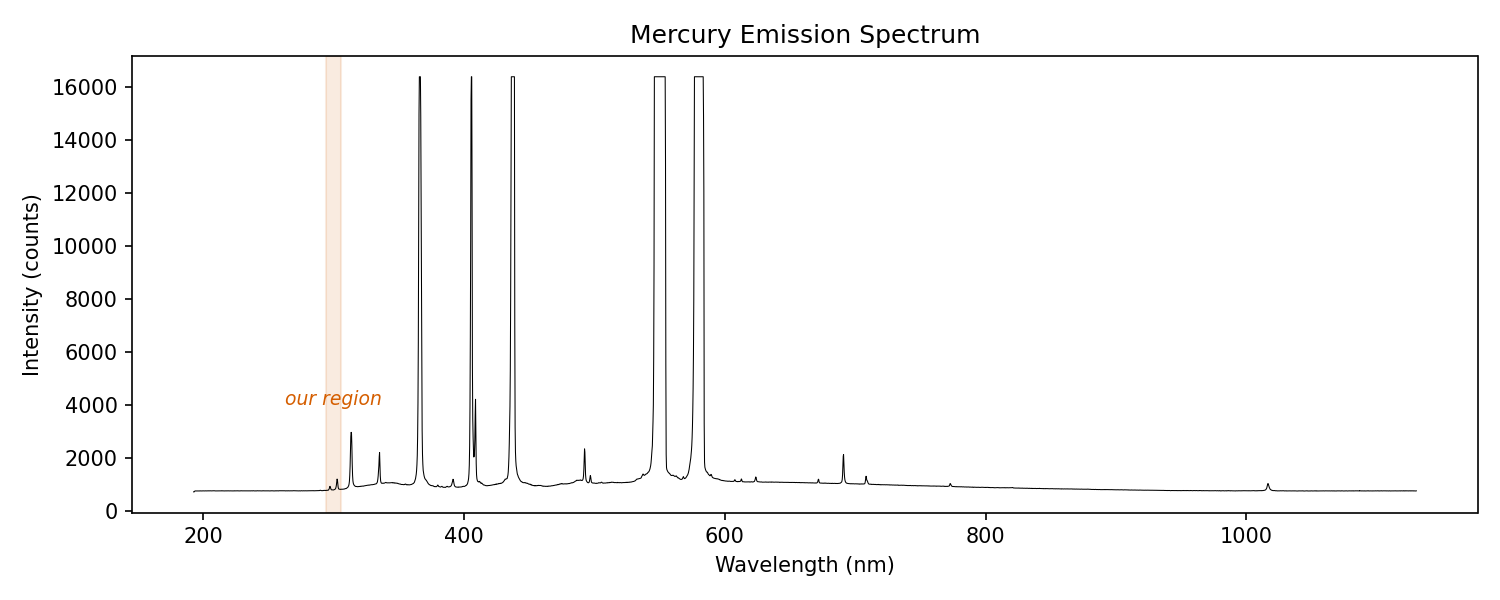
\includegraphics[width=\columnwidth, height=0.35\textheight, keepaspectratio]{data/mercury_full_spectrum.png}

\vspace{4pt}
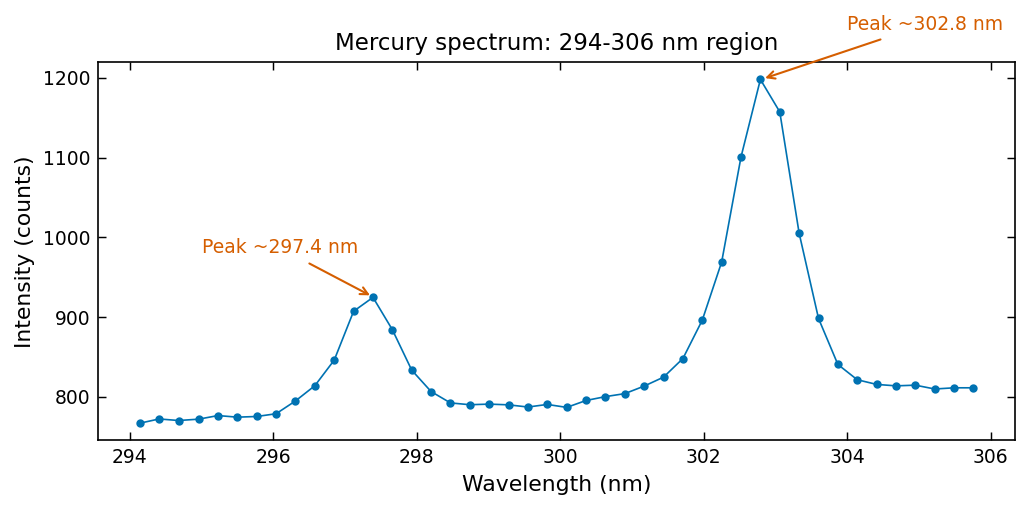
\includegraphics[width=\columnwidth, height=0.35\textheight, keepaspectratio]{data/mercury_300nm_region.png}
\vfill
\end{column}
\end{columns}
\end{frame}

% =============================================================================
% SLIDE 5 --- Separate single-Gaussian fits
% =============================================================================
\begin{frame}[fragile]{Step 3: Fit each peak separately}

\footnotesize
You can also fit each peak individually with \texttt{gaussian\_baseline}:

\begin{columns}[t]
\begin{column}{0.48\textwidth}
\textbf{Peak at 297.3 nm:}
\begin{lstlisting}[style=pysmall]
mask1 = (data.x > 296) & (data.x < 299)
r1 = fit(data.x[mask1], data.y[mask1],
         model="gaussian_baseline",
         sigma=data.y_err[mask1])
\end{lstlisting}

\scriptsize
Amplitude $= 137 \pm 4$, Centre $= 297.33 \pm 0.015$~nm, $\chi^2_\nu = 0.10$

\vspace{2pt}
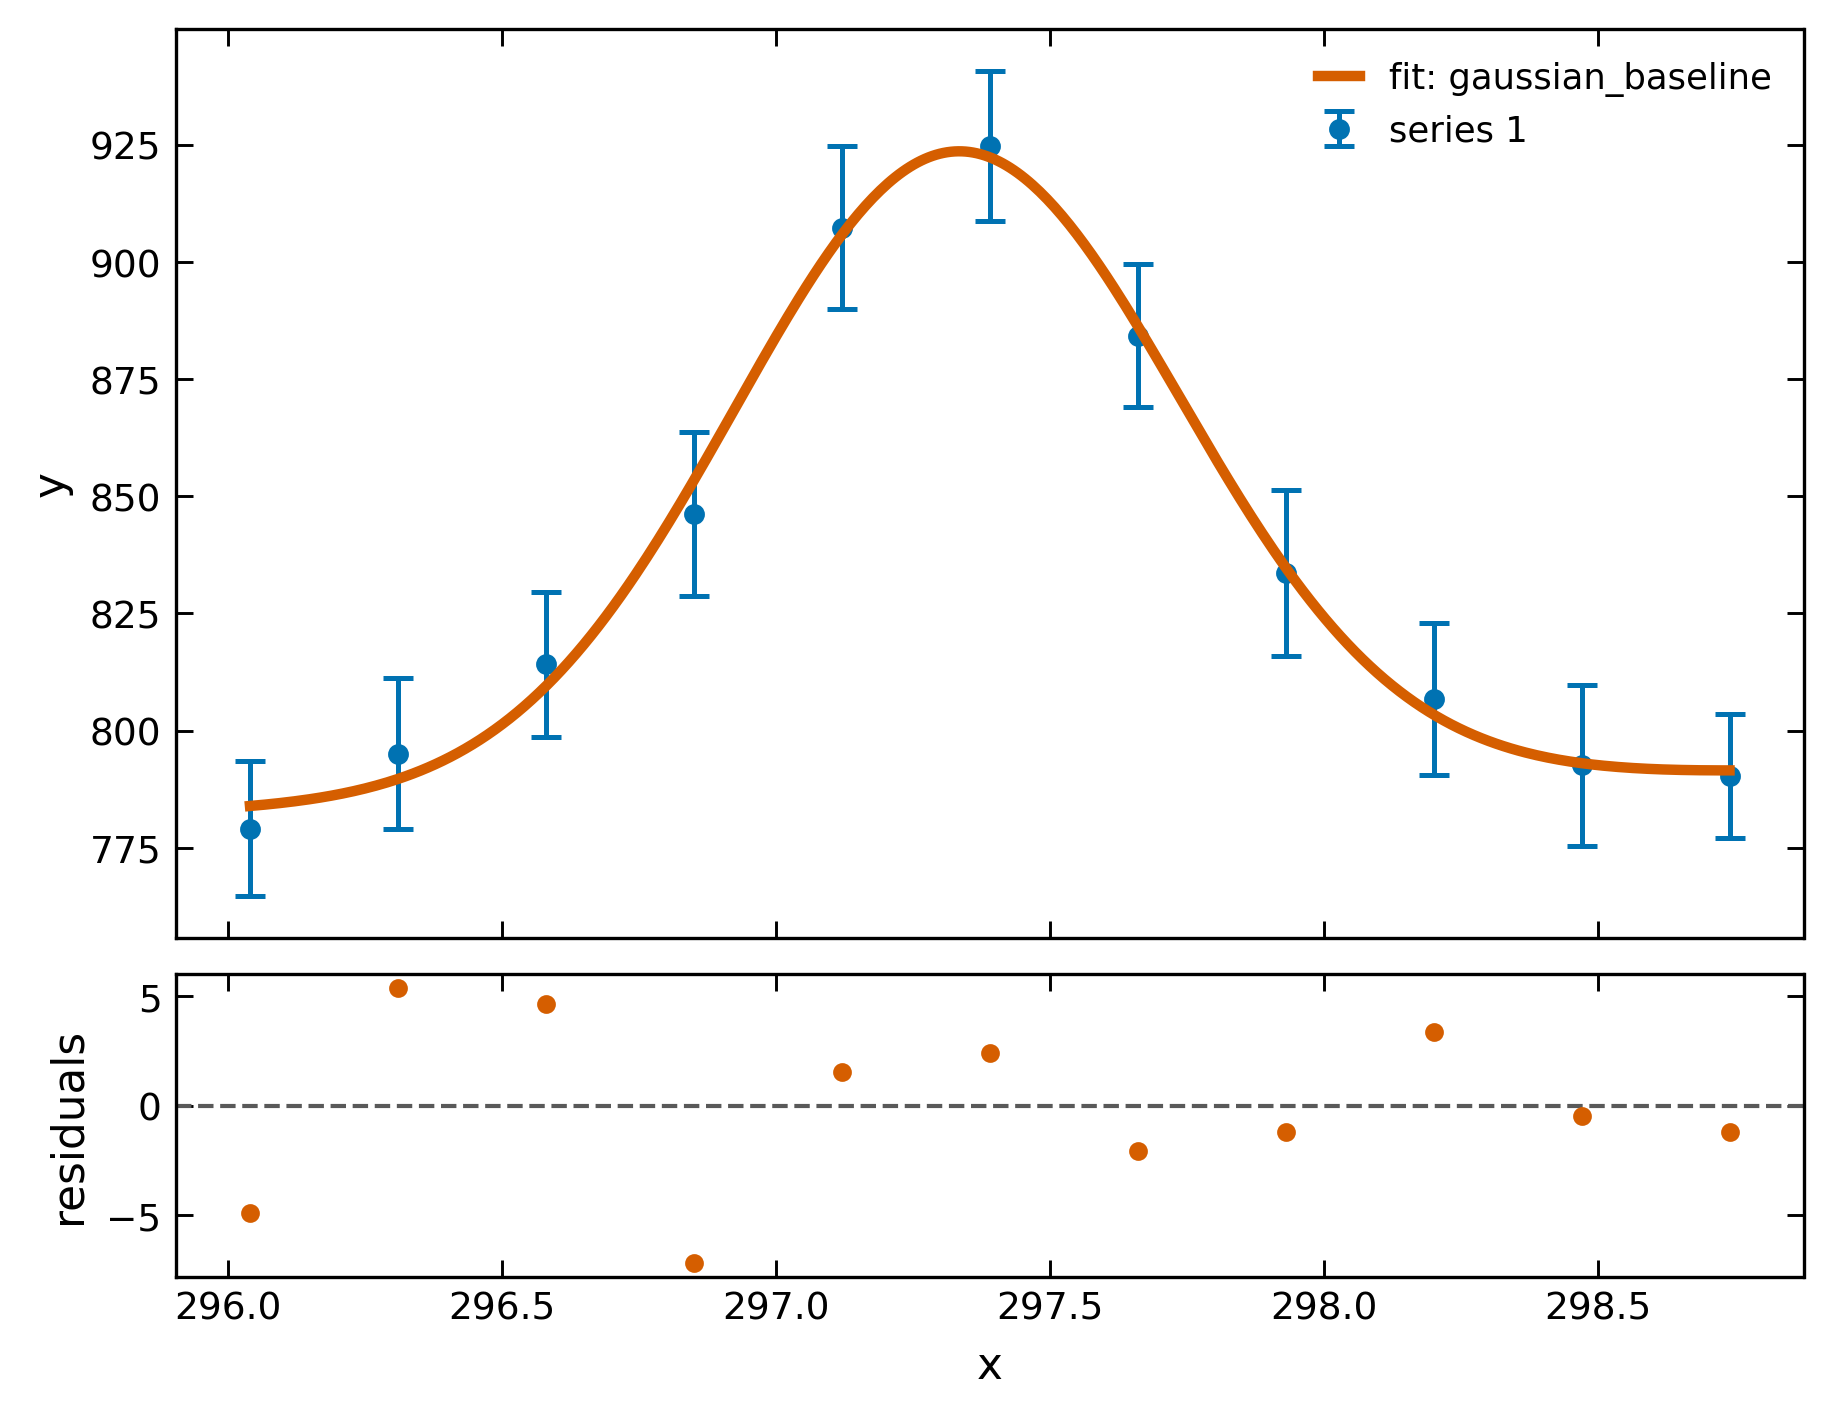
\includegraphics[width=\columnwidth]{data/mercury_297nm_single_fit.png}
\end{column}
\begin{column}{0.48\textwidth}
\textbf{Peak at 302.8 nm:}
\begin{lstlisting}[style=pysmall]
mask2 = (data.x > 301) & (data.x < 305)
r2 = fit(data.x[mask2], data.y[mask2],
         model="gaussian_baseline",
         sigma=data.y_err[mask2])
\end{lstlisting}

\scriptsize
Amplitude $= 374 \pm 8$, Centre $= 302.83 \pm 0.012$~nm, $\chi^2_\nu = 0.40$

\vspace{2pt}
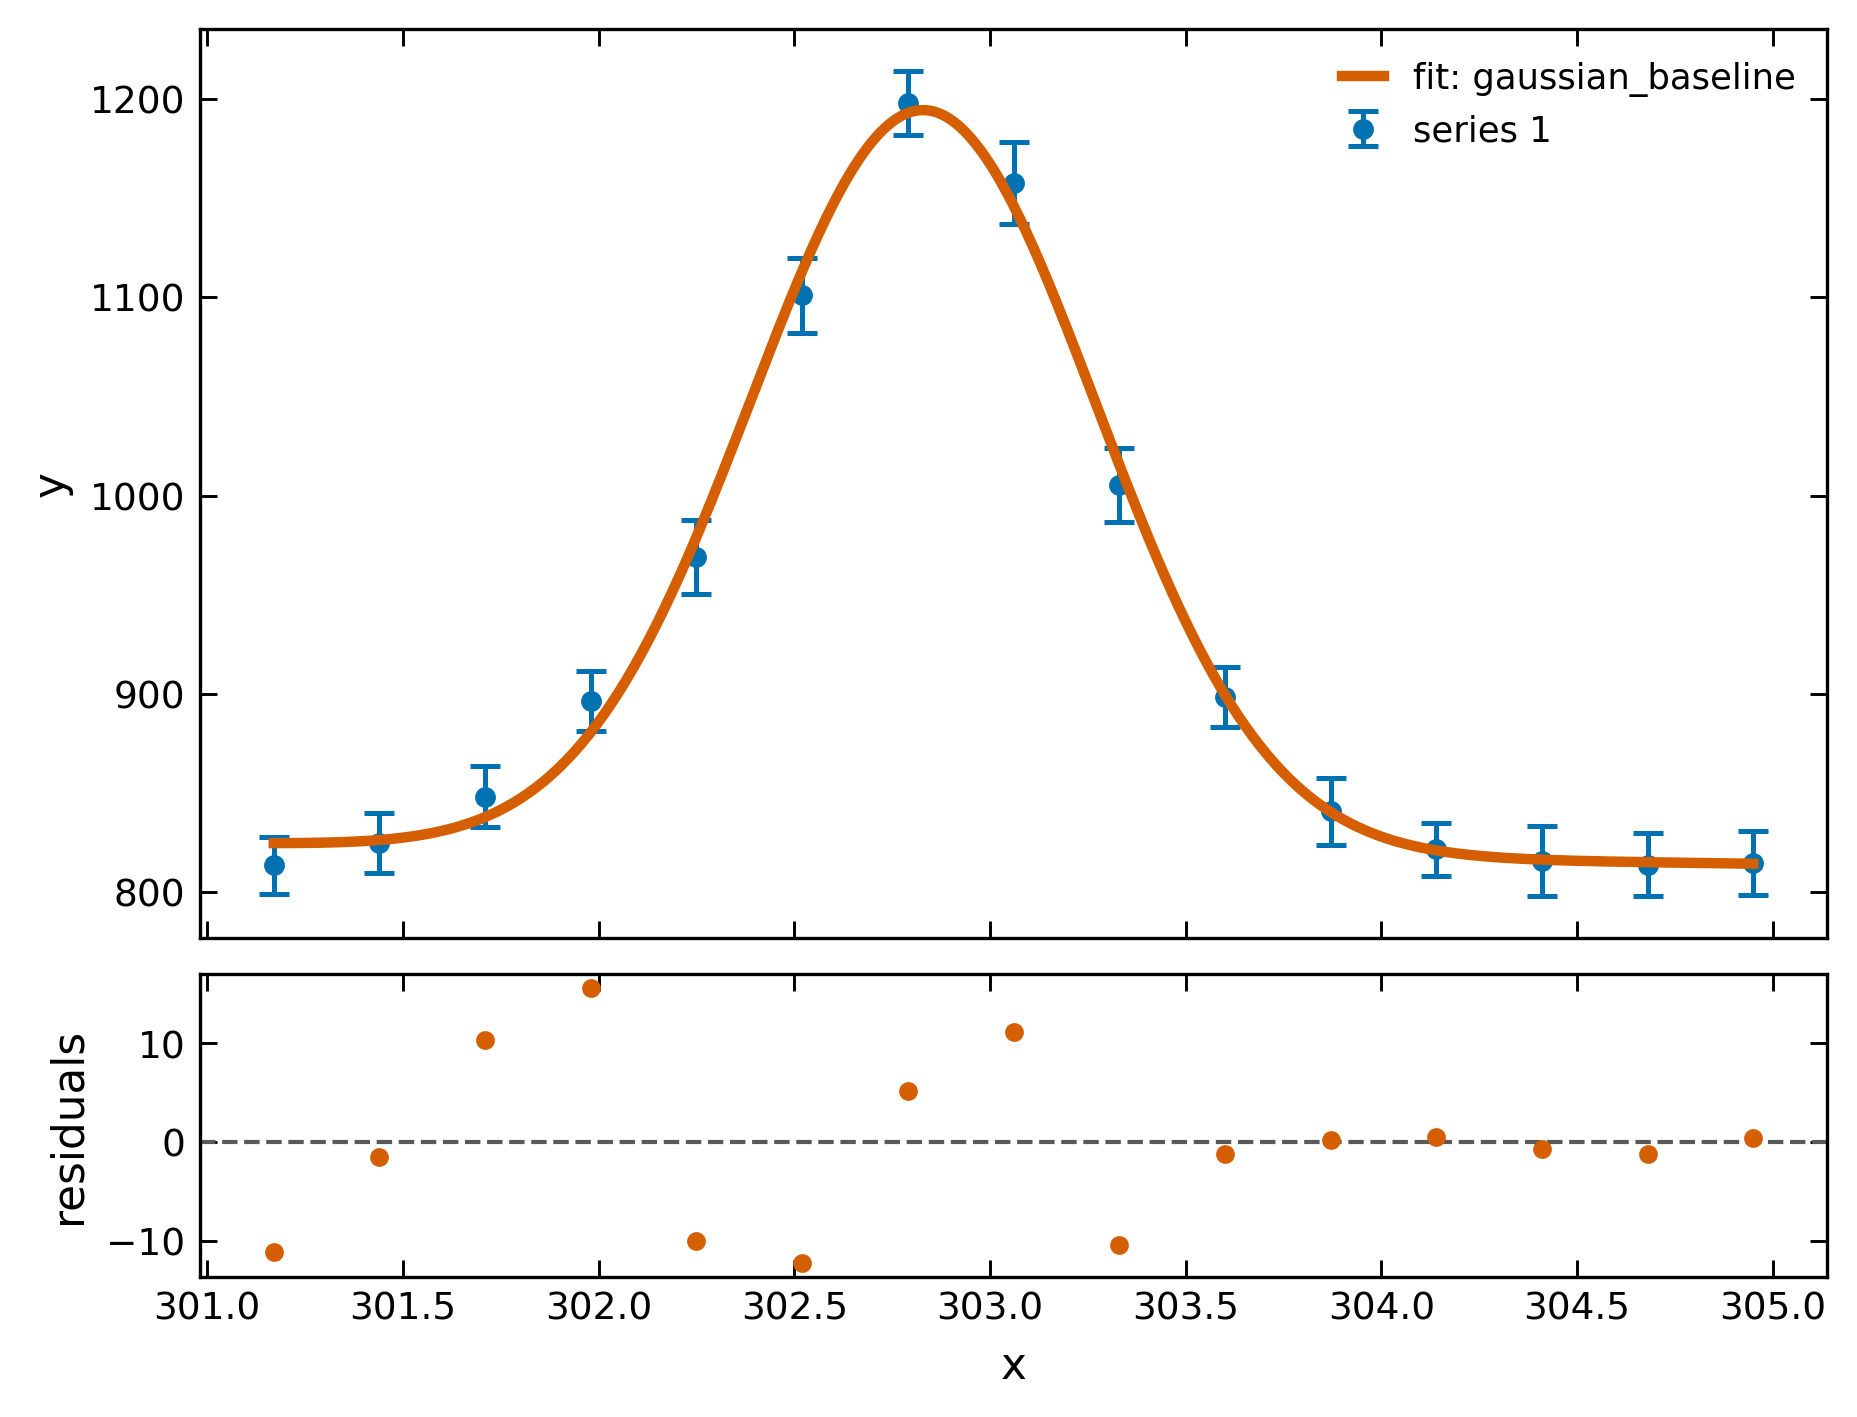
\includegraphics[width=\columnwidth]{data/mercury_302nm_single_fit.png}
\end{column}
\end{columns}

\vspace{4pt}
\tiny
Separate fits are simpler but ignore the overlap. Use a joint model when
peaks are close enough to share baseline.
\end{frame}

% =============================================================================
% SLIDE 6 --- Custom two-Gaussian model
% =============================================================================
\begin{frame}[fragile]{Step 4: Define a custom two-Gaussian model}

For overlapping peaks, write a model function or use the built-in equation:

\[
I(\lambda) = A_1 e^{-(\lambda-\mu_1)^2/2\sigma_1^2}
           + A_2 e^{-(\lambda-\mu_2)^2/2\sigma_2^2}
           + m\lambda + b
\]

\begin{lstlisting}[style=pysmall]
def two_gaussians_baseline(x, a1, m1, s1, a2, m2, s2, m, b):
    g1 = a1 * np.exp(-0.5 * ((x - m1) / s1) ** 2)
    g2 = a2 * np.exp(-0.5 * ((x - m2) / s2) ** 2)
    return g1 + g2 + m * x + b
\end{lstlisting}

\begin{lstlisting}[style=pysmall]
result = fit(x_pk, y_pk, model=two_gaussians_baseline,
             sigma=e_pk,
             p0={"a1": 150, "m1": 297.4, "s1": 0.6,
                 "a2": 400, "m2": 302.8, "s2": 0.6,
                 "m": 0, "b": 780})
\end{lstlisting}

\medskip
\texttt{p0} provides initial guesses:
\begin{itemize}
    \scriptsize
    \item \texttt{a1}, \texttt{a2}: approximate peak heights
    \item \texttt{m1}, \texttt{m2}: approximate centre wavelengths
    \item \texttt{s1}, \texttt{s2}: approximate widths (half-width at half-height $\times 0.85$)
    \item \texttt{m}, \texttt{b}: baseline slope and offset
\end{itemize}
\end{frame}

% =============================================================================
% SLIDE 7 --- Interpret results
% =============================================================================
\begin{frame}[fragile]{Step 5: Interpret the fit results}

\begin{columns}[t]
\begin{column}{0.50\textwidth}
\begin{lstlisting}[style=pysmall]
FitResult: two_gaussians_baseline
  a1 = 138.4 +/- 6.8
  m1 = 297.33 +/- 0.024 nm
  s1 = 0.418 +/- 0.025 nm
  a2 = 382.6 +/- 6.8
  m2 = 302.82 +/- 0.010 nm
  s2 = 0.472 +/- 0.009 nm
  m  = 3.79 +/- 0.34
  b  = -342.9 +/- 103.3
  reduced chi2 = 0.301
  p = 1
\end{lstlisting}
\end{column}
\begin{column}{0.46\textwidth}
\vspace{4pt}
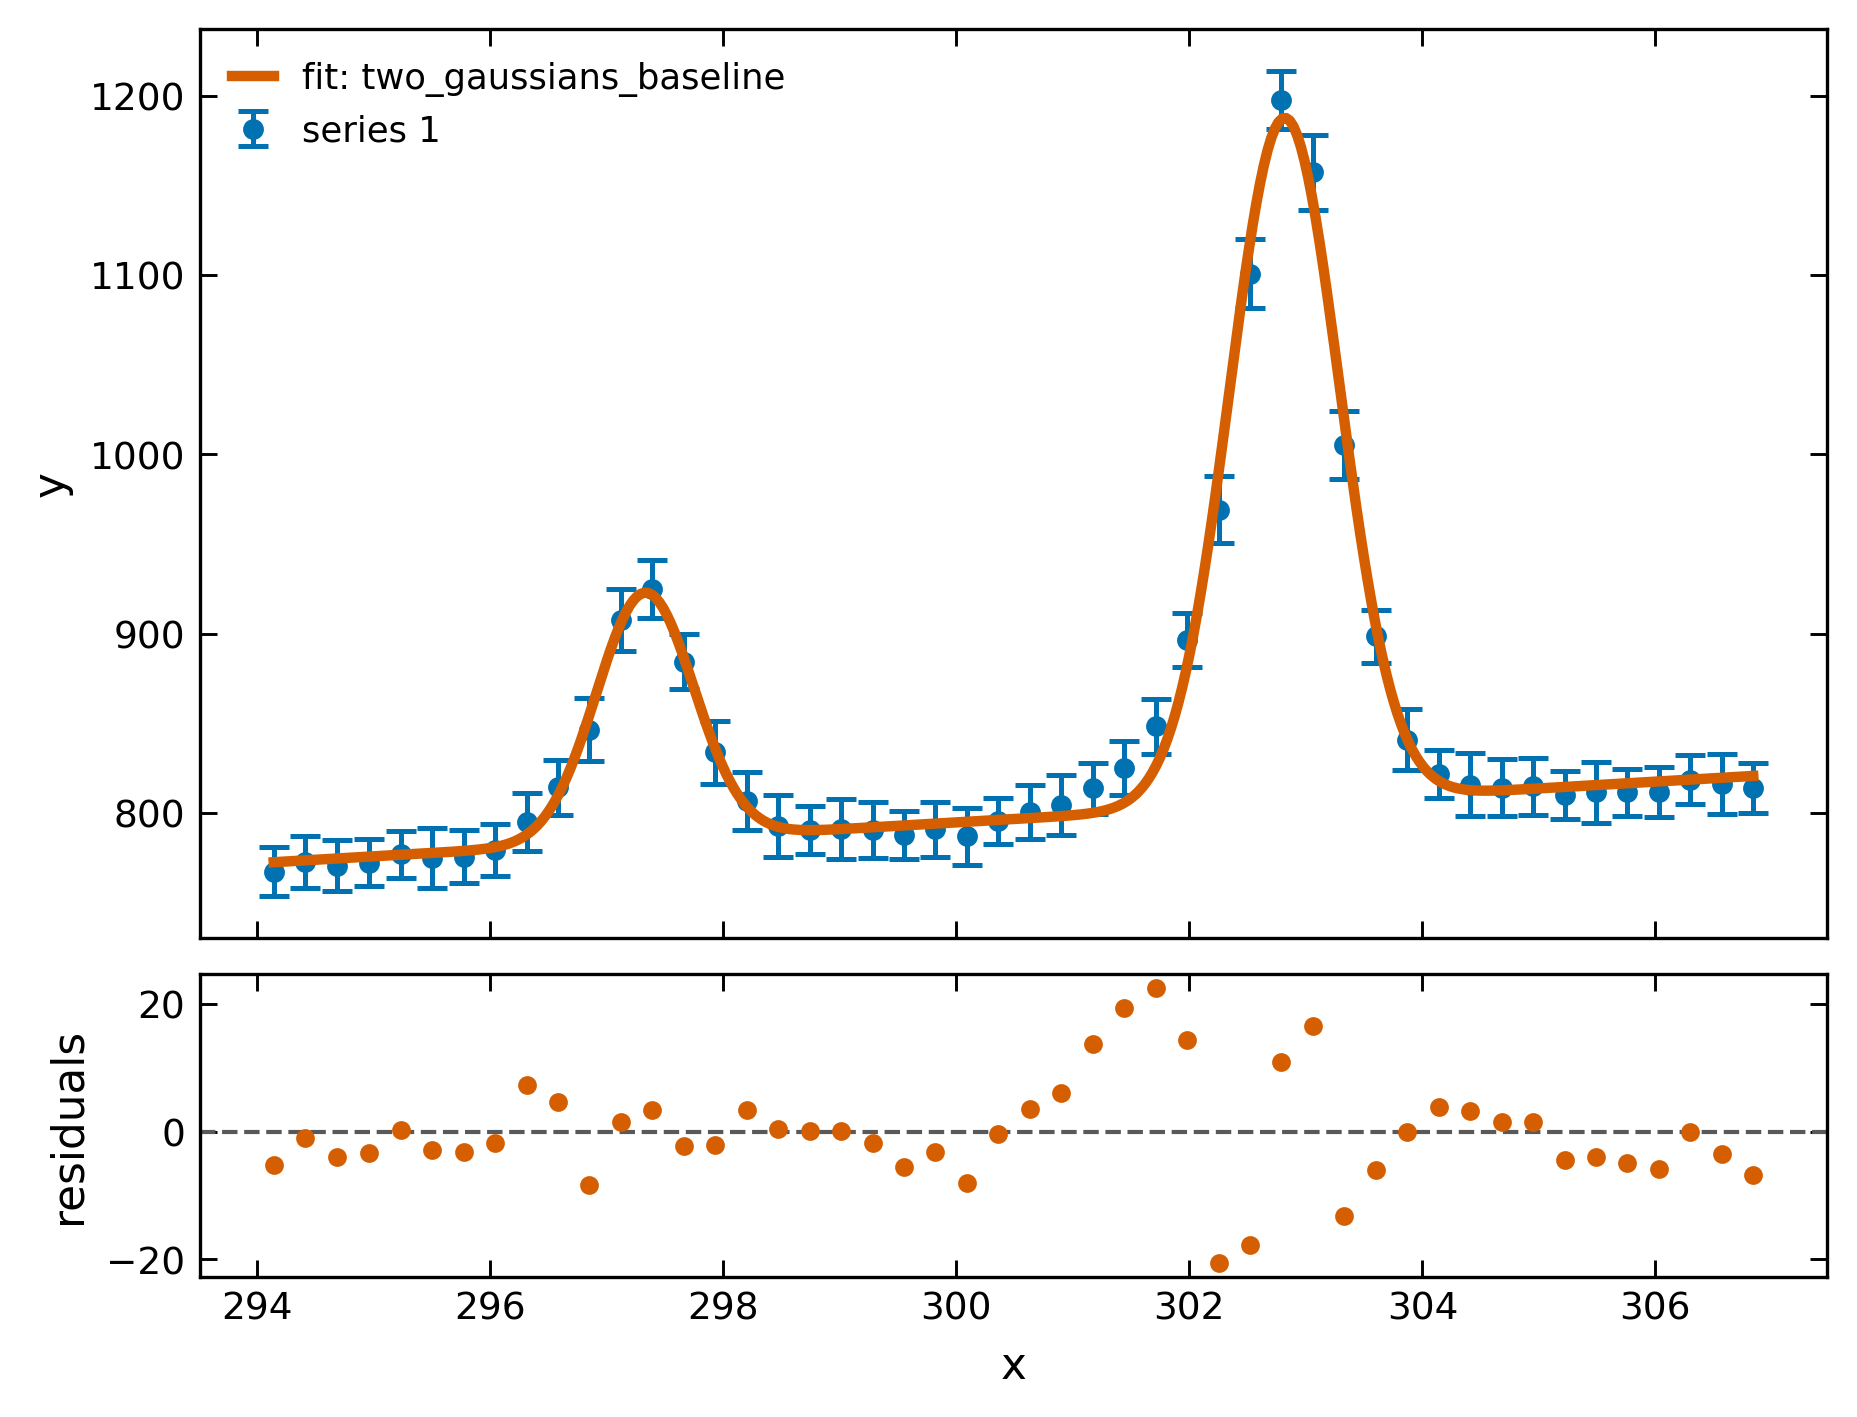
\includegraphics[width=\columnwidth]{data/mercury_300nm_bimodal_fit.png}

\end{column}
\end{columns}

\vspace{6pt}
\begin{tcolorbox}[colback=labgreen!5, colframe=labgreen!80, size=small]
Both peaks are well resolved: $\chi^2_\nu = 0.30$ (close to~1).
Peak centres have sub-0.03~nm precision!
\end{tcolorbox}
\end{frame}

% =============================================================================
% SLIDE 8 --- What chi-squared tells you
% =============================================================================
\begin{frame}{What $\chi^2$ tells you}

\[
\chi^2_\nu = \frac{1}{\nu}\sum_i \left(\frac{y_i - f(x_i)}{\sigma_i}\right)^{\!2}
\]

\begin{itemize}
    \item $\chi^2_\nu \approx 1$: residuals are consistent with the uncertainties
    \item $\chi^2_\nu \gg 1$: model is wrong \textbf{or} errors are underestimated
    \item $\chi^2_\nu \ll 1$: errors may be overestimated
\end{itemize}

\medskip
Our $\chi^2_\nu = 0.30$ is slightly below 1, suggesting our error bars
are a bit conservative. This is still a \textbf{good fit} -- the residuals
scatter randomly around zero with no systematic pattern.

\medskip
\begin{tcolorbox}[colback=laborange!5, colframe=laborange!80, size=small]
What if $\chi^2_\nu \gg 1$? Either the model is wrong (e.g.\ trying a single
Gaussian on two overlapping peaks) or the uncertainties are too small.
Always inspect the residuals to tell the difference!
\end{tcolorbox}
\end{frame}

% =============================================================================
% SLIDE 9 --- Visualise
% =============================================================================
\begin{frame}[fragile]{Step 6: Visualise with residuals}

\begin{lstlisting}[style=pystyle]
from labfit import plot_fit

p = plot_fit(result, show_residuals=True)
p.save("mercury_300nm_bimodal_fit.png")
\end{lstlisting}

\medskip
\texttt{plot\_fit} produces data with error bars, the best-fit curve,
and a \textbf{residual sub-panel} showing $(y_i - f(x_i))/\sigma_i$.

\centering
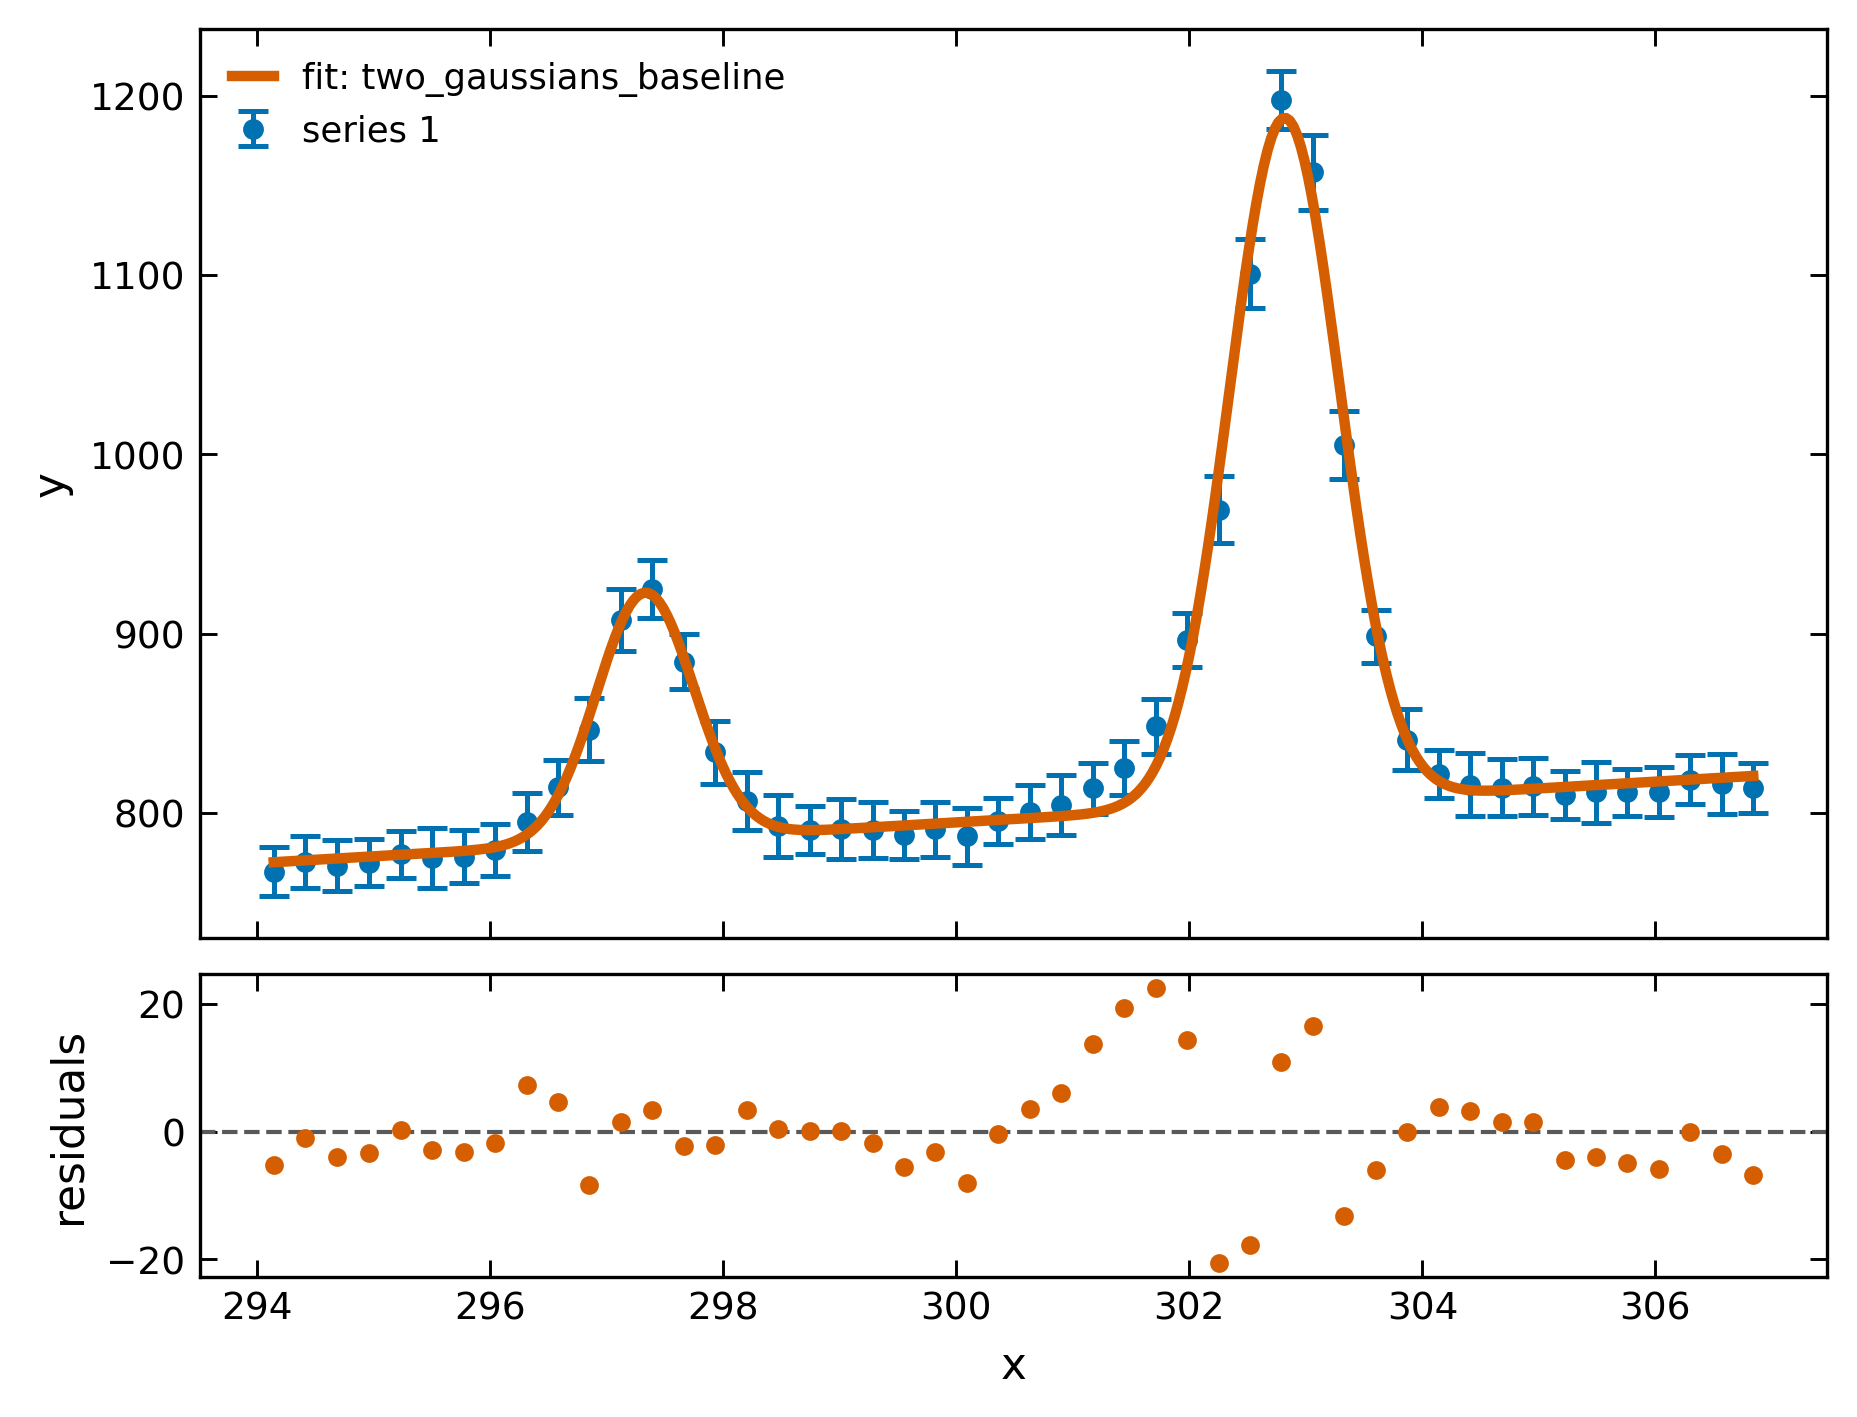
\includegraphics[width=0.42\textwidth]{data/mercury_300nm_bimodal_fit.png}
\end{frame}

% =============================================================================
% SLIDE 10 --- Practical tips
% =============================================================================
\begin{frame}{Practical tips}

\begin{enumerate}
    \item \textbf{Always plot first.} Know your data shape before
          choosing a model.
    \item \textbf{Zoom in.} Fit one peak (or one small group) at a time.
    \item \textbf{Give good \texttt{p0}.} The optimiser is not magic.
    \item \textbf{Examine residuals.} Patterns mean your model is
          missing something.
    \item $\chi^2 \gg 1$ can mean underestimated errors, not a bad fit.
    \item \textbf{Read the uncertainties.} If error $>$ value, the
          parameter is unconstrained.
    \item \textbf{Document everything.} Save the code, fit window, and
          parameter table -- future you will thank present you.
\end{enumerate}
\end{frame}

% =============================================================================
% SLIDE 11 --- Summary
% =============================================================================
\begin{frame}[fragile]{Summary}

\begin{tcolorbox}[colback=labgreen!5, colframe=labgreen!80, size=small, title=You can now:]
\begin{itemize}
    \item Load spectral CSV data with \texttt{labfit.io.load\_csv}
    \item Select a region of interest (NumPy masking)
    \item Fit Gaussian ($+$ baseline) to an emission line
    \item Define a custom multi-Gaussian model
    \item Interpret parameters, uncertainties, and $\chi^2$
    \item Spot unreliable fits and know what to try next
\end{itemize}
\end{tcolorbox}

\vspace{6pt}
\textbf{5-line workflow:}

\begin{lstlisting}[style=pystyle]
from labfit.io import load_csv
from labfit import fit, plot_fit
data = load_csv("mercury_int10s.csv", x_col="wavelength_nm", y_col="intensity")
result = fit(data, model="gaussian_baseline")
plot_fit(result).save("my_fit.png")
\end{lstlisting}

\vspace{4pt}
\centerline{Happy fitting! \quad $\star$ \quad
\url{https://github.com/matthewjdoyle/labfit}}

\end{frame}

\end{document}
